% Initialisation
\documentclass[english,12pt]{scrartcl}
\usepackage[]{babel}
% Input is utf8
\usepackage[utf8]{inputenc}
% Enables headers and footers
\usepackage[]{scrpage2}
% Lets us colour table cells
\usepackage[table]{xcolor}
% Allows todo list and todos
\usepackage[]{todonotes}
% Makes links in contents hyperlinked
\usepackage{hyperref}
% Make references appear in our table of contents
\usepackage[nottoc,numbib]{tocbibind}
% Allows us to put landscape sections of the document
\usepackage{pdflscape} % \usepackage{lscape} %Use escape for printing (doesn't rotate the pdf page)
% Provides a glossary
\usepackage[toc]{glossaries}
% Used for source code syntax highlighting
\usepackage{minted}
% Stops \texttt{} text from overflowing
\usepackage[htt]{hyphenat}
% Allows us to force figure positioning
\usepackage{float}

% Minted configuration
\usemintedstyle{vs}
\newminted{cpp}{tabsize=0,linenos,bgcolor=white!95!black}

% Gives us pretty diagrams
\usepackage{tikz}
\usetikzlibrary{calc,fit,positioning,chains,decorations.pathreplacing,shapes,backgrounds}

% Document Title and Author
\title{
\includegraphics[width=0.75\textwidth]{./Logo/NUClear-logo}~\\[1cm] Design Document}
\author{2013 Final Year Project}

% Header and Footer
\pagestyle{scrheadings}
\ihead{\today}
\chead{}
\ohead{NUClear Design Document}
\ifoot{}
\cfoot{}
\ofoot{\pagemark}

% Requirements custom commands
\newcommand{\requirement}[1]{\textit{#1}}

% Skip line rather then indent paragraphs
\setlength{\parindent}{0.0in}
\setlength{\parskip}{0.1in}

% Start of document
\begin{document}
	\maketitle

	\vfill
	{\large
		\begin{description}
			\item [Status:] Release 1
			\item [Version:] 1.0
		\end{description}}

	\clearpage
	\tableofcontents
	\clearpage

	\section{Summary}
		\subsection{Project Background}
			The NUbots are a team of Software Engineers and Computer Scientists from the University of Newcastle who build software for robots in order to compete in RoboCup.
			RoboCup is an international competition that pits two teams of robots against each other in an soccer competition with the goal of challenging humans by the year 2050.

			The robot software system has been developed at the University of Newcastle by the NUbots since 2002 and has changed robots three times between 2002-2013 initially starting with the four-legged \emph{Sony AIBO} robots followed by the two legged \emph{Aldebaran Nao} and as of 2011 they are now using the \emph{Robotis DARwIn-OP}.
			The NUbots have also been successful at taking home the coveted RoboCup trophy twice in their career.

			The existing robot software was developed by separating different processing systems (Vision, Localisation, Kinematics, etc...) into their own code modules that communicate using ad-hoc mechanisms on a per-module basis.
			Unfortunately constant developer churn and a long-lived code base have resulted in a system that contains very impressive algorithms that are hindered by a myriad of complicated and confusing communication methods.

			Our team was asked to develop a solution to this communication problem by restructuring the architecture around the individual systems to allow them to communicate in a \emph{Simple}, \emph{Efficient} and \emph{Unified} way.

			We were also asked to assist with some of the fundamental problems with the existing architecture that have arisen from changing platforms and hardware over the years.
			Our ultimate goal is to provide a system that allows the NUbots to focus on the amazing algorithms and research without spending a disproportionate amount of time writing code to move data from system to system.

		\subsection{Recommend Solution}
			After careful analysis of the existing system we determined that it is prohibitively expensive to incrementally refactor the existing code base.
			However we have also determined that the algorithmic parts of the system can be separated from the architecture without a large investment of labour.

			Based on these observations we decided to build a new architecture from the ground up while migrating the existing algorithms into the new system as it is built.
			It was important to ensure that we only made changes to algorithmic code when necessary to decouple it from the old architecture while still leaving the algorithms intact.

			\subsubsection{Technologies}
				A key requirement set out by the NUbots team was to make it possible to easily replace components of the system with functional equivalents.
				For example it should be possible to replace the system that reads camera frames from the hardware with one that reads frames from a file without changing the rest of the system.

				To facilitate this we looked at a number of different communication strategies to identify architectures that promoted \emph{loose coupling} which is a measure of how dependent components are on each other.
				Architectures that are \emph{loosely coupled} have been shown to support easy drop-in replacement of modules provided they require/provide the same information.

				Currently the consensus in the robotics world is to utilise message passing systems whereby modules communicate by sending and receiving packets of data known as \emph{messages} without knowing where they are sending/receiving message to/from.

				During our research it was clear that the majority of mature robotic systems were built with a message-driven architecture in mind.
				Currently \textbf{Robot Operating System (RobotOS)} is the de-facto standard platform for robotics research.
				RobotOS uses a message passing system and was considered very heavily as a replacement for the existing architecture.

				Unfortunately RobotOS has a very high performance penalty to support message passing which was completely unacceptable for resource-starved platforms such as the Darwin.
				Other existing robot systems such as \textbf{Dynamic Data eXchange (DDX)} and \textbf{Pack Service Robotic Architecture} also suffer from the same issues. It seemed that all contemporary robotic systems have decided to trade performance for message passing and cross-language compatibility.

				Our team decided to leverage our C++ skills to build an alternative system named \textbf{NUClear} that provides message passing capabilities (and more) that are orders of magnitudes faster then the competing systems.
				Once we had a proof-of-concept it was decided to use the NUClear architecture as the basis for the new NUbots architecture. NUClear is covered extensively in the Architecture Overview.

	\section{NUClear Design}
		NUClear is the C++ library that we designed to enable developers to write modular systems that communicate using messages.
		Modules are kept ignorant of each other and only know about the messages they send/receive.
		This allows us to transparently drop in different producers/consumers without modifying the entire system.

		NUClear was designed to replace the most common method of communication in the existing architecture known as the Blackboard.
		Blackboards are a shared global memory store that all modules use to communicate by writing data to the blackboard and assuming it is read by the next module.
		Our design makes it easy to transition from similar globally accessible data to a message based event-driven architecture.
		NUClear is also capable of replacing other methods of communication currently in use in the existing system such as direct function calls.

		Our goal was to make a system that allows programmers to easily send/receive information between modules using mechanisms that are \textbf{Fast}, \textbf{Reliable} and \textbf{Intuitive}.

		\subsection{Features}
			\subsubsection{Simple API}
				It is critical that NUClear have a simple and intuitive interface that didn't require weeks of study to achieve productivity with.
				As such NUClear is designed to be usable by second year software students who have a basic understanding of C++.
				With that in mind we ensured that there was a single well-defined function for the two key features of the architecture: sending and receiving messages. Sending is accomplished using the \textbf{Emit} function while receiving is accomplished using the \textbf{On} function.

				NUClear is designed around these two functions. \textbf{On} provides mechanisms to indicate that you are interested in a particular piece of information.
				\textbf{Emit} correspondingly allows you to provide information to the system.

				The major benefit of having such a small API is understandability.
				Instead of having to memorise tens or hundreds of functions you just need to remember two key functions and you have the full power of NUClear at your fingertips.
				This makes it easy for new programmers to learn and understand.

			\subsubsection{Simple utilization of system resources}
				Another requirement derived from resource-constrained environments is the need to easily utilise the full power of the platform you run on.
				This is primarily achieve by introducing \textbf{Transparent Multi-threading} which automatically uses every physical core available on the system without the developer needing to fiddle with threading primitives.

				When a message is sent in the system the central coordination object known as the \textbf{PowerPlant} takes ownership of it.
				From this point forward no modules can modify the message and only have read-only access to it.
				The PowerPlant then executes callbacks, known as reactions, that are subscribed to this message.
				Each reaction gets a immutable reference to the original message and can perform any read operations on it.

				Immutability is the key that allows us to transparently multi-thread the system.
				We know that multiple reactions will want to read the data and if we can guarantee that they don't modify it then we can
				run the reactions in parallel without worrying about race conditions.
				By forcing immutability we can move all threading logic directly into NUClear allowing developers to concentrate on their modules instead of threading problems.

				In most cases multi-threading will be completely transparent.
				However it is still important that the developers understand that they are working in a multi-threaded environment.
				If a single module shares data between two reactions and those reactions could run in parallel then the shared data will
				need to be secured with a thread-safe mechanism such as a mutex.
				NUClear also provides functionality to let the user specify that certain reactions should not be run in parallel which can be used to solve threading concerns.

			\subsubsection{Low Performance Penalty}
				In order to meet our clients requirements it is essential that message routing is performed as quickly as possible.

				Because of this we have opted not to use technologies that incur large performance penalties such as text-based message serialisation (XML, JSON).
				Instead we have chosen a direct binary representation for messages passed within a single process.

				We also need to minimise the amount of time it takes to send a message.
				To achieve this NUClear uses modern C++ features enabling us to perform partial message routing at compile time.
				Normally when you send a message there is a message broker executes some code to find the systems that are interested in a particular message.
				This system usually uses a number of intermediate steps to locate the appropriate messages.

				Additionally we are able to perform compile time memory allocation using template meta-programming to determine at compile time how much space is needed for messages.
				We can then use that information to preallocate the space before the program runs giving us the ability to send an arbitrary number of messages in O(1) time.

				Thanks to the mechanism used to allocate messages optimising compilers are also able to reason about the memory allocation of the messages at compile time which gives the compiler the opportunity to apply a number of powerful optimisations to how messages are sent.

				Our tests show that NUClear is able to operate between 1000-7000 times faster then competing message passing systems such as CORBA or RobotOS.

			\subsubsection{Statistics, Logging and Traceability}
				In complex system it can become very difficult to determine what the system is actually doing and why it's doing it.
				The NUbots team made it clear that the ability to get per-module statistics and logs would be invaluable in tackling the challenges of robotic software development.

				To facilitate this NUClear is built with powerful statistics and logging tools.
				NUClear stores runtime statistics about each modules and provides mechanisms to get the information logs on a per-module or per-reaction basis.
				By integrating these features into the NUbots architecture we are able to provide a large amount of useful information to assist them with debugging or understanding the robot system.

				Additionally if an error occurs it's possible to capture the input that caused the error and replay it on the module.
				This functionality can be used to develop a powerful array of tests that accurately simulate real-time scenarios.

				For example: If the robot kicks the ball and you expected it to do something else you can capture the inputs that made it decide to kick and replace them at your convenience.
				It's also possible to encode the captured input into a unit test which can be automatically replayed.
				This lets the NUbots team verify that the bug has been fixed and ensure that future changes don't cause a regression.

		\subsection{Architecture}
			NUClears architecture consists of three major building blocks: the \textbf{PowerPlant}, \textbf{Reactor}s and \textbf{Reaction}s.

		\subsection{Component Overview - Power Plant}
			The PowerPlant is the central message system through which all modules communicate.
			Message routing is actually performed at compile time but from an API point of view the system still communicates through the PowerPlant.

			The PowerPlant has three main responsibilities which are split up into named subsystems called \emph{Masters}.

			In general when a message is emitted it is first cached by the CacheMaster.
			The ThreadMaster then spawns a new thread and then tells the ReactorMaster to execute any reactions that are subscribed to that particular message.
			The ReactorMaster then uses the CacheMaster to retrieve the message data and then invokes the reactions with the message data.

			\subsection{CacheMaster}
				The CacheMaster is responsible for ensuring that there is enough storage for all uses of a particular message.
				In most cases this means it needs to ensure there is space allocated for at least one instance of every message.
				However some extensions may require that more then the most recent message be cached and the CacheMaster also needs to account for that.

				The CacheMaster is fed the minimum allowable size for a particular message buffer at compile time by the PowerPlant.
				Internally the CacheMaster uses a data structure known as the TypeMap which is a compile-time mapping between types and instances of that type.
				By using this structure we are able to perform all cache sizing calculations at compile time and ensure that all messages are accounted for.

				Additionally the CacheMaster is the primary memory management facility for all messages in the system.
				The CacheMaster keeps track of references to messages and automatically cleans up memory when it is not longer used.
				It's possible for other systems to take ownership of data from the CacheMaster but it must be explicitly requested and is rare to see in regular modules.

				Routing of messages is technically a responsibility of the CacheMaster.
				However, we don't actually send messages for in-process communication in NUClear.
				Instead messages are stored in the CacheMaster which then provides references to the ReactorMaster that are sent to the reactions.
				For the user this still looks like message routing but behind the scenes this approach gives us massive speed advantages of conventional copy-based routing.

			\subsection{ThreadMaster}
				The ThreadMaster is responsible for multi-threading and task scheduling.
				It contains an internal thread pool that contains a number of workers.
				Each worker executes a reaction using the ReactorMaster and then requests a new task from a blocking queue.

				When the system is started the ThreadMaster spins up a number of ThreadWorkers and places them in a thread pool.
				These workers then request reaction tasks from a job queue that is populated by the ReactorMaster.
				When a new job comes in it is taken by the first available ThreadWorker who then executes it.
				Additionally ThreadWorkers record statistics about how long a particular task took and store them in a ReactionStats object.

			\subsection{ReactorMaster}
				The ReactorMaster handles the logic relating to \emph{On} and \emph{Emit} directly.
				It can be thought of as the glue that holds Reactors, the ThreadMaster and the CacheMaster together.

				When a Reactor calls Emit behind the scenes it is actually calling on the ReactorMaster to resolve the request.
				The ReactorMaster uses the CacheMaster to cache the data that was emitted.
				The ReactorMaster then loops through all reactions in the reaction list for that message type and adds a task to the ThreadMaster for each reaction.

				Additionally the ReactorMaster can also execute reactions directly in the main thread.
				This is useful for tasks that are faster then the overhead of moving data to a new thread and is sometimes used for very quick reactions.

				Internally all reactions are stored in a data structure similar to the TypeMap called a TypeList.
				A TypeList is a compile-time list of instances of a particular type. This list can be iterated over extremely quickly and allows us to perform subscriber lookup in O(1) time.
				Combining this with the already fast CacheMaster is what gives us a lot of our speed advantage of RobotOS or DDX.

		\subsection{Component Overview - Reactor and Reaction}
			A Reactor encapsulates a single module that can send and receive messages.
			Each Reactor contains a number of Reactions which are a single function that is run in response to new data.
			Reactions take immutable references to messages as arguments which provide a strong multithreading guarantee that allows multiple reactions accessing the same data to be run simultaneously.

			Reactors are the primary entry point to the NUClear API.
			It is expected that each module in a system will extend from NUClear::Reactor and use it's member functions to send and receive messages.
			By subclassing from Reactor you gain access to the two main NUClear API functions \emph{On} and \emph{Emit}.
			Additionally you also gain access to \emph{Log} which provides per-reactor logging capabilities.

			\subsubsection{On}
				\emph{On} subscribes a reaction to particular message.
				On also has a number of arguments that customise what data it receives and triggers on.
				On takes a number of template arguments to specify the type of data you are interested in.
				The two major ways of requesting data are using \emph{Trigger} and \emph{With}.
				\emph{Trigger} tells NUClear that you want to execute a callback when new data for a particular type comes in.
				This is called "Triggering" on a type.
				For example:

				\begin{cppcode}
					// Arguments are immutable (const) and references (no copying)
					void processImage(const Image& data) {
					    // Do something with the image data here.
					}

					on<Trigger<Image>>(processImage);
				\end{cppcode}

				\emph{With} tells NUClear that you are interested in something but you don't want to trigger on it.
				It's designed to solve the case where you want to do something when Image data comes in but you also want access to Motor Position data.
				It can be used like this:

				\begin{cppcode}
					void processImage(const Image& data, const MotorPositions& motors) {
					    // Do something with image and motor data here
					}

					on<Trigger<Image>, With<MotorPositions>>(processImage);
				\end{cppcode}

				\emph{With} also allows you to request multiple chunks of data so you're not limited to just a single extra piece of data.
				Consider the case where you need Image, Vision and Localization data (such as in behaviour) triggering on new Vision frames:

				\begin{cppcode}
					void processBehaviour(const Vision& vision, const Image& image,
					    const Localization& loc) {
					    // Do something with vision, image and localization here
					}

					on<Trigger<Vision>, With<Image, Localization>>(processBehaviour);
				\end{cppcode}

			\subsubsection{Emit}
				\emph{Emit} is responsible for sending data to the rest of the system.
				Internally it sends data to the PowerPlant which then uses the various masters to send the message on its way.

				The most basic use of emit looks like this:

				\begin{cppcode}
					// We have a unique pointer to the data we want to send.
					std::unique_ptr<MyData> myData = std::make_unique<MyData>();

					// send the data to the world!
					emit(std::move(myData));
				\end{cppcode}

				This basic example sends MyData to the entire system.
				Anything that Triggers on MyData will then be executed on a worker thread.

				Emit also provides primitives for sending to different scopes.
				The most common different scope is the Networked scope which sends messages to other robots on your network.
				For example:

				\begin{cppcode}
					// We have a unique pointer to the data we want to send (again).
					std::unique_ptr<MyData> myData = std::make_unique<MyData>();

					// Send the data to the network!
					emit<Scope::NETWORK>(std::move(myData));
				\end{cppcode}

				As you can see sending data to the network is almost as simple as sending data normally.
				By default this won't send data to internal modules.
				If you want to send data to both the network and locally you can use multiple scopes like so:

				\begin{cppcode}
					// We have a unique pointer to the data we want to send (again).
					std::unique_ptr<MyData> myData = std::make_unique<MyData>();

					// Send the data to the network!
					emit<Scope::LOCAL, Scope::NETWORK>(std::move(myData));
				\end{cppcode}

				\begin{figure}[p]
					\centering
					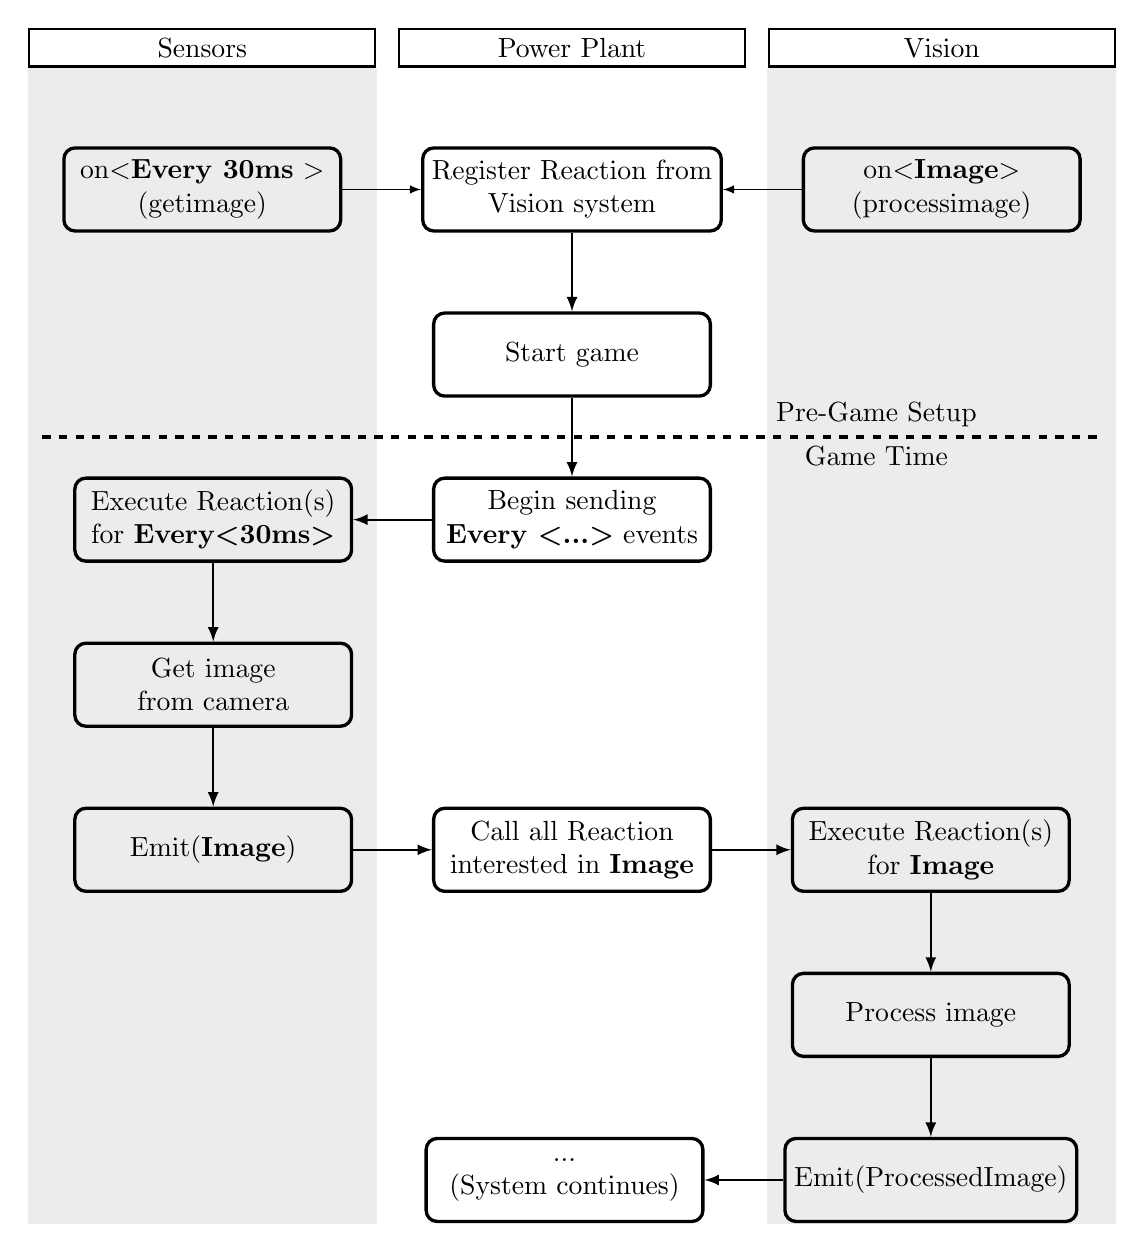
\begin{tikzpicture}[>=latex,
						block/.style={
							rectangle,
							rounded corners,
							draw=black, very thick,
							minimum height=3em,
							minimum width=10em,
							align=center
						},
						header/.style={
							rectangle,
							draw = black, thick,
							minimum height=1.2em,
							minimum width=12.5em,
							align=center
						},
						every join/.style={->, thick},
						chained/.style={every node/.style={on chain}}]

						\begin{scope}[start chain=going below, chained]

							% Draw the Register node and setup the following blocks to have arrows
							\node [block,join] (register) {Register Reaction from \\ Vision system};
							\begin{scope}[start branch=on going right, every join/.style={<-}]
								\node [block,join] (onimage) {on\textless \textbf{Image}\textgreater
								\\(processimage)};
							\end{scope}

							% Draw the on Every node
							\begin{scope}[start branch=on going left, every join/.style={<-}]
								\node [block,join] (onevery) {on\textless \textbf{Every 30ms}
								\textgreater\\(getimage)};
							\end{scope}

							% Start game node
							\node[block,join] (start) {Start game};

							% In Game every node
							\node [block, join] (runtimeStart) {Begin sending\\\textbf{Every
								\textless ...\textgreater} events};

							% Sensor Reactors node
							\node [block, join, on chain=going left] {Execute Reaction(s) \\for
								\textbf{Every\textless 30ms\textgreater}};

							% Get Camera Image Node
							\node [block, join] {Get image\\from camera};

							% Emit Node
							\node [block, join] {Emit(\textbf{Image})};

							% Image Call Node
							\node [block, join, on chain=going right] {Call all Reaction\\interested
								in \textbf{Image}};

							% Execute Reactions Node
							\node [block, join, on chain=going right] {Execute Reaction(s)\\for
								\textbf{Image}};

							% Process Image Node
							\node [block, join] {Process image};

							% Emit Processed Image node
							\node [block, join] {Emit(ProcessedImage)};

							% Continuation Node
							\node [block, join, on chain=going left] (final) {...\\(System continues)};
						\end{scope}

						\coordinate (setuplineA) at ([xshift=-18em]$ (start) !.5! (runtimeStart) $);
						\coordinate (setuplineB) at ([xshift=18em]$ (start) !.5! (runtimeStart) $);
						\coordinate (setupTextPoint) at ([xshift=11em]$ (start) !.5! (runtimeStart) $);

						%% Setup dividing line and text
						\node [above] at (setupTextPoint) {Pre-Game Setup};
						\node [below] at (setupTextPoint) {Game Time};
						\draw [dashed, ultra thick, shorten >= -0.4cm, shorten <= -0.4cm]
							(setuplineA) -- (setuplineB);

						%% Add headers for the three threads
						\node [header,above=of onevery] (sensorsHeader) {Sensors};
						\node [header,above=of register] {Power Plant};
						\node [header,above=of onimage] (visionHeader) {Vision};

						%% Add the column backgrounds for Sensors and Vision
						\begin{scope}[on background layer]
							\filldraw [gray!15] (sensorsHeader.south west) rectangle
								(sensorsHeader.east |- final.south);
							\filldraw [gray!15] (visionHeader.south west) rectangle
								(visionHeader.east |- final.south);
						\end{scope}
					\end{tikzpicture}
						\caption {A flowchart example of how \textbf{On}, \textbf{Emit} and \textbf{Every} work}
						\label{fig:OnAndEmitExample}
				\end{figure}

			\subsubsection{Log}
				\emph{Log} provides a mechanism to log information against a particular reaction.
				This provides logging information that is per-reaction rather then system-wide giving greater traceability.

				Logging is implemented internally using the standard iostream operator$<<$ mechanism.
				This means that anything you can log with std::cout can also be logged with NUClear's log function.

				Log accepts an infinitely long set of arguments, concatenates them together and adds them as a single log entry to the reaction you are in.
				Consider the following example:

				\begin{cppcode}
					void processImage(const Image& image) {
					    log("Got data: ", image.data);
					}

					on<Trigger<Image>>(processImage);
				\end{cppcode}

				In the previous example the "Got data" message is attached to the processImage reaction allowing us to determine the exact context the message occurred in.
				This makes it easy to filter through thousands of log messages to find the relevant information.

		\subsection{Extension}
			The NUClear API has been designed so that it is extensible.
			Despite the fact that there are only two functions that are available in the system, it is possible to add the ability for users to alter the effects of these functions is defined cases.
			This allows users of the NUClear framework to add new functionality to the core system without having to modify the complex metaprograms.
			There are four anchor points at which an extension to the NUClear framework can be installed to modify the system.

			The first of these is the TriggerType extension.
			This extension is able to change the type that a message is triggered on.
			For example, if a message of a particular type is emitted, it can cause the running of a function with a different function signature.
			This is useful for cases where one type is requested, but that type is based on another type.
			For example if a type of \texttt{Increment<int>} were a theoretical type, then it may be triggered when an int is emitted rather then the requested \texttt{Increment<int>} type.

			The second possible anchor point is the Exists anchor point.
			This anchor point is used when a function should be run because a type exists within a Trigger or With statement.
			For example, in the configuration system if a Configuration type exists, then that type must be registered for events with the configuration system.
			This allows it to generate events that are used in the configuration system simply by the type existing in the system.

			The third possible extension point is to override the Get function for a particular type.
			This allows changing of how data is retrieved when a particular type is requested.
			For example, if the type that is requested is accessed through a database and not NUClear, then by overriding how that information is obtained, the user can influence the system for that type.

			The final method of overriding is through Emit.
			Emit can be overridden for any type or controller, this allows the user to control how the system uses data that is emitted.
			This can be used to implement functionality such as networking, or communication with a database, or simply to intercept data elements and modify them before they are sent to the rest of the system.

		\subsection{Smart Types}
			Through the use of the extensibility provided by NUClear, it is possible to implement special types which have been named Smart Types.
			These types when used are able to perform manipulations and other non standard behaviour in the system.
			These allow the system to be more useful as it provides an expansion of functionality as part of the API and not an additional module.
			A number of these Smart Types have already been implemented as a core part of the NUClear framework, However it is also possible to implement them as a user of NUClear

			\subsubsection{Every}
				In real-time systems it's common to have a number of systems that need to execute periodically.
				In our analysis of the existing NUbots architecture we found several examples of systems that need to do something periodically.
				For example Camera frames need to be read 30 times per second and Motors need to be read and written to 50 times per second.

				The way this is accomplished in the existing NUbots architecture is to manually set up a thread and have it block until the polling period is up.
				Unfortunately this approach ties up a CPU thread doing almost nothing and wastes valuable hardware resources.

				NUClear provides an alternative mechanism that allows you to execute code periodically without tying up a CPU core.
				You can set up a reaction on a time event and NUClear will ensure that your reaction is called periodically.
				Instead of busy waiting the system will run other tasks while the period task is waiting which ensures that CPU cycles are not wasted doing nothing.

				The manner in which the functionality was implemented was through a smart type.
				This smart type is called Every and consists of an integer to wait for, and a time unit for the integer.
				This allows the system to combine all polling that is necessary in one place and perform it as a part of the NUClear API.

				\begin{cppcode}
				// Example of Every
				on<Trigger<Every<50, std::chrono::milliseconds>>>(function);
				\end{cppcode}

			\subsubsection{Last}
				In systems it is often very important to not only look at the most recent information but also prior information.
				This is useful in scenarios where data must be operated on over a series of time.
				However in NUClear alone there is only a method to access the most recent element, and not prior elements.
				As the information which is provided is not owned by the reactor, the only available way would be to copy the information into local memory and manage it.

				In order to solve this problem, a smart type called Last is available in the NUClear system.
				This smart type is able to access the references held by the CacheMaster and provide a list of these to the modules that request them.
				This allows the system to access the previous elements without having to deal with storing the information locally or the overhead of copying this data.

				The Last smart type consists of the number of elements to return, as well as the type to be returned.
				It will trigger whenever a type of the requested type is requested and will also get the previous number of elements.
				It does this by accessing the raw shared pointer which is stored in the CacheMaster.
				This allows it to ensure the lifetime of the data without having to copy the information itself.

				\begin{cppcode}
				// Example of Last
				on<Trigger<Last<10, Image>>>(function);
				\end{cppcode}

			\subsubsection{Networked}
				One of the pain points cited in the old system was networking.
				To address this NUClear provides facilities to send messages over the network.
				Networking is implemented through the Extension API and provides a good case study of the power available to users of the extension API.

				The Networking extension introduces a new emit scope which can be used to send message, as shown in the Reactor overview:

				\begin{cppcode}
					// Send a message to the network
					emit<Scope::NETWORK>(message);

					// Send a message locally and to the network
					emit<Scope::LOCAL, Scope::NETWORK>(message);
				\end{cppcode}

				Internally the Networking extension uses the ZeroMQ library to handle connection management.
				ZeroMQ handles the creation of connections to other robots and handles transfer of binary data between machines.

				We also utilize google protocol buffers to serialise/deserialise messages.
				Google Protocol Buffers is a object serialisation library that serialises objects into a binary format.
				Compared to XML and JSON, protocol buffers produce smaller messages more quickly and allow us to rapidly serialise messages for transfer over the network.

				In order to receive networked messages NUClear provides a Network smart type that specifies you are looking for networked data:

				\begin{cppcode}
					void processNetworkImage(const Network<Image>& image) {
					    // Do something with the image from the network here.
					}

					// Trigger on images from the network
					on<Trigger<Network<Image>>>(processNetworkImage);
				\end{cppcode}

				The \texttt{Network<Image>} object also contains information identifying the robot it was sent from allowing you to filter data by its source.

				% Networking diagram
				\begin{figure}[H]
					\centering
					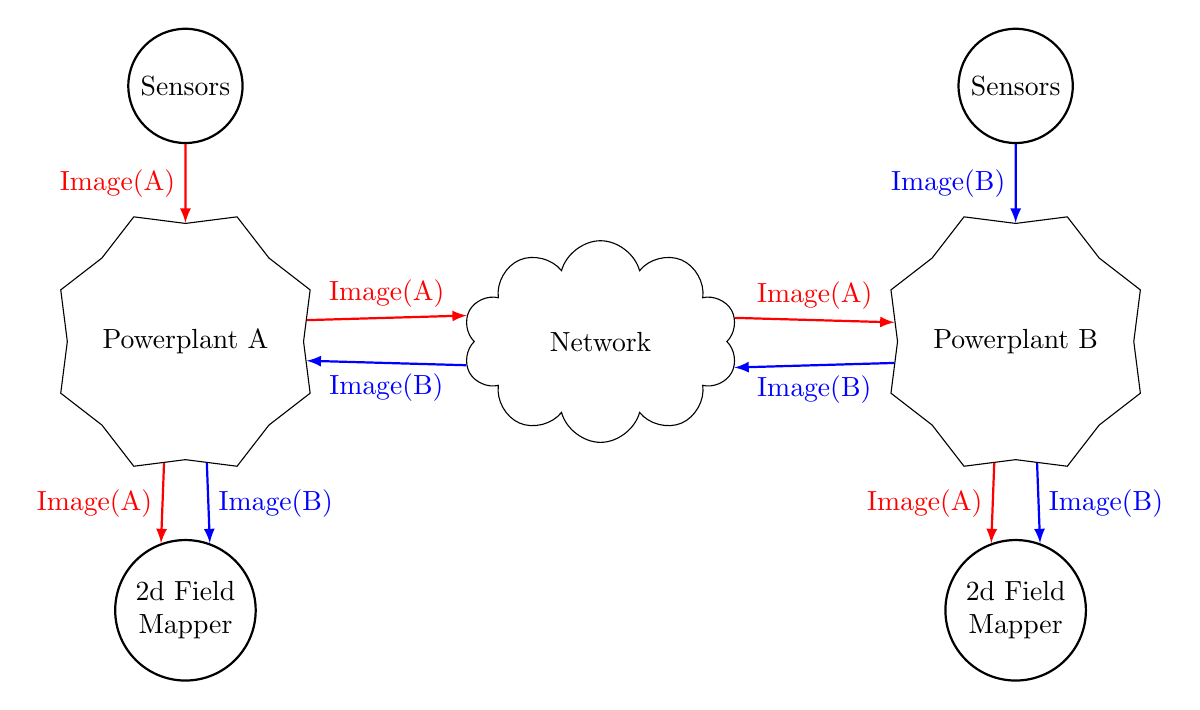
\begin{tikzpicture}[x=15em,y=5em,>=latex,
						A/.style={red},
						B/.style={blue},
						reactor/.style={draw, circle, thick},
						write/.style={->,thick},
						read/.style={<-,thick}]

						%%% Left Power Plant
						\node at (0, 0) [draw,star,star points=8,star point ratio=0.875,minimum width=3cm] (plantA) {Powerplant A};
						\node [above=of plantA,reactor] (sensorsA) {Sensors};
						\node [below=of plantA,reactor,align=center] (fieldmapperA) {2d Field\\Mapper};
						\path [A, write] (sensorsA) edge node[A,left] {Image(A)} (plantA);
						\path [A, read] (fieldmapperA.110) edge node[left] {Image(A)} (plantA.260);
						\path [B, read] (fieldmapperA.70) edge node[right] {Image(B)} (plantA.280);

						%%% Right Power Plant
						\node at (2, 0)
							[draw,star,star points=8,star point ratio=0.875,minimum width=3cm]
							(plantB){Powerplant B};
						\node [above=of plantB,reactor] (sensorsB) {Sensors};
						\node [below=of plantB,reactor,align=center] (fieldmapperB) {2d Field\\Mapper};
						\path [B, write] (sensorsB) edge node[left] {Image(B)} (plantB);
						\path [A, read] (fieldmapperB.110) edge node[left] {Image(A)} (plantB.260);
						\path [B, read] (fieldmapperB.70) edge node[right] {Image(B)} (plantB.280);

						%%% Network & Network Connections
						\node at (1, 0) [draw,cloud,cloud puffs=10,minimum width=3.5cm]
						(network) {Network};

						%% Plant A connections
						\path [A, write] (plantA.10) edge node[A, above] {Image(A)} (network.169);
						\path [B, read] (plantA.-9) edge node[B, below] {Image(B)} (network.190);

						%% Plant B connections
						\path [A, read] (plantB.171) edge node[A, above] {Image(A)}  (network.10);
						\path [B, write] (plantB.190) edge node[B, below] {Image(B)} (network.-11);
					\end{tikzpicture}
					\caption {An example of how robots can communicate camera data over a network to
						build a 2d map of the field}
						\label{fig:NetworkExampleDiagram}
				\end{figure}

		\section{Putting it all together}
			We've seen examples of all the major features of NUClear but what does an actual module look like?
			To answer this question we've got an example for you right here!
			The following module is designed to make the robots eyes strobe when it hears a beat:

			\begin{cppcode}
				// PartyStrobe.h
				class PartyStrobe : NUClear::Reactor {
				    public:
				        PartyStrobe(NUClear::PowerPlant* plant);
				};

				// PartyStrobe.cpp
				#include "PartyStrobe.h"
				PartyStrobe::PartyStrobe(NUClear::PowerPlant* plant)
				: NUClear::Reactor(plant) {
				    // Every time we hear a beat we want to max out the eye values.
				    on<Trigger<Beat([this](const Beat& beat) {
				        // We've detected a beat; set the eyes to max
				        auto newEyes = std::make_unique<EyeLED>();

				        // We're taking 10% out of the eyes every 100 milliseconds
				        newEyes->r = 0xFFF;
				        newEyes->g = 0xFFF;
				        newEyes->b = 0xFFF;

				        emit(std::move(newEyes));
				    });

				    // Every 1/10th of a second we want to lower the eye intensity
				    // so that it's noticeable when it strobes back up.
				    on<Trigger<Every<100, std::chrono::milliseconds>>,
				       With<EyeLED>>([this](const time_t&, const EyeLED& eyeLED) {
				        // Construct a new EyeLED message to change the eye colour.
				        auto newEyes = std::make_unique<EyeLED>();

				        // We're taking 10\% out of the eyes every 100 milliseconds
				        newEyes->r = eyeLED->r - (0xFFF / 10);
				        newEyes->g = eyeLED->g - (0xFFF / 10);
				        newEyes->b = eyeLED->b - (0xFFF / 10);

				         // Send the message out
				         emit(std::move(newEyes));
				    });
				}
			\end{cppcode}

	\section{NUClear Powered NUbots}
		The NUClear framework provides a central point around which the NUbots project has been
		reconstructed. This has facilitated many improvements both on an architectural and
		implementation level.

		The pre-existing NUbots codebase is divided into subsystems, however their boundaries are
		often poorly defined. The use of both direct function calling between subsystems and
		shared data through the blackboard have led to difficulty in separating otherwise
		unrelated functionality. To solve this problem we have redefined and solidified the
		boundaries between subsystems by creating smaller, more cohesive modules. This is a
		significant task for larger subsystems such as vision, as such parts of the port are
		not yet complete.

		Efforts have been made, when possible, to improve the quality of code as it is being
		transitioned. These include removing dead code that remained from previous hardware
		platforms, adding documentation, adopting modern C++ practices such as the use of smart
		pointers and replacing large numbers of preprocessor macros in favour of templates and
		constants.

		The changes to the overall architecture and improvements in testing and documentation
		should improve the NUbots' maintainability and extensibility and allow new team members
		to begin working on the project with a much shorter induction period.


		\subsection{Architecture}
			Modules are the primary architectural units of the NUClear-based NUbots system. Each
			one is intended to implement a single feature or task. They have no knowledge of or
			interaction with other modules except through NUClear messages. A module consists of
			a single NUClear Reactor subclass (with the same name as the module itself), any
			supporting source files, a set of unit tests, configuration files and documentation.

			Messages that modules use to communicate are defined in a separate, shared component.
			This also includes a small collection of utility classes and functions.

			By separating functionality into modules we gain the ability to unit test in isolation,
			which was largely impossible in the previous design. The project's build scripts
			automatically compile unit tests alongside the modules and can run them as a batch.

			The \emph{pimpl} (private implementation) idiom is used to avoid specifying
			implementation details such as library dependencies and private member data in header
			files when not necessary.


		\subsection{Orchestration/Roles}
			NUClearPort uses a collection of CMake build scripts to automate the build process.
			Each module is built separately into a library, both enforcing the requirement for
			them to be independent and allowing them to be combined into executables at
			link-time.

			One of the desired features of the new NUbot architecture was the flexibility to
			change existing behaviour or create entirely new behaviour as easily as possible. To
			this end the concept of a \textbf{role} has been created. The roles system is our
			implementation of orchestration, a term most commonly associated with service-oriented
			architectures, whereby complex systems are built by coordinating a range of disparate
			components.

			A role represents an executable built from a specific subset of modules. When a role
			is defined, the build system automatically generates a C++ source file containing code
			to create a Power Plant and install each of the specified modules in the given order.
			It then builds an application from it, linking against the libraries for the modules
			that it uses.

			This design allows large parts of the code to be shared (for example, the hardware
			interface layers and script execution engine) while other parts are swapped in and
			out. Switching between two compatible modules (with the same inputs and outputs)
			requires editing only the roles list and rebuilding. This also allows for a subset of
			modules to be integration tested without including other irrelevant code, or
			producing a special build including extra logging and debugging modules.


		\subsection{Modules}

			\subsubsection{AubioBeatDetector}
				This module finds the beat in music as it plays using the Aubio library's
				tempo-finding algorithm.

				On receipt of a \texttt{SoundChunkSettings} message containing the sample format
				of the sound, this module sets up an Aubio tempo tracking context and begins
				receiving \texttt{SoundChunk} messages. As it detects beats, it sends out
				\texttt{Beat} messages.

				It depends on the libaubio library, and requires that one of the audio input
				modules be installed to provide it with data.


			\subsubsection{AudioFileInput}
				This is one of the audio input modules; as it emits the same messages as
				AudioInput both can be used interchangeably. It reads sound from a file and emits
				it in short, regular-sized chunks. These are generated in real time, as if the
				sound was being recorded from the microphone.

				The audio file to be loaded is determined by a setting in the module's
				configuration file. Once successfully opened, AudioFileInput emits a
				\texttt{SoundChunkSettings} message to inform downstream modules of the sample
				format (bit depth, sample rate, number of channels)	and number of samples that
				will be present in subsequent sound chunks. After this, it periodically emits
				\texttt{SoundChunk} messages containing the PCM samples of the sound until
				the end of the file is reached.

				AudioFileInput depends on the libsndfile library to decode sound files, and
				requires that the configuration system module be installed in order to read its
				configuration file.


			\subsubsection{AudioInput}
				This is one of the audio input modules; as it emits the same messages as
				AudioFileInput both can be used interchangeably. It records sound from the
				machine's default audio input device (generally a microphone) and emits it in
				regular-sized chunks.

				On startup, AudioInput attempts to open the system's default audio input device
				using its highest available sample rate, native channel count and 16-bit depth.
				Assuming this is successful it then emits a \texttt{SoundChunkSettings} message
				to inform downstream modules of the sample format and size of upcoming chunks.
				After this, it begins emitting \texttt{SoundChunk} messages containing PCM from
				the input device.

				AudioInput depends on the librtaudio library to communicate with audio devices.


			\subsubsection{BeatDetector}
				This module finds the beat of music as it plays using an algorithm based on signal analysis using basic Fourier transformations.

				BeatDetector starts working when it receives a \texttt{SoundChunkSettings} message
				indicating the format of upcoming sound chunks, which allows it to prepare its
				buffers. Samples are then received from \texttt{SoundChunk} messages and placed
				into a 10 second sliding window, which is analysed to find beats. Whenever one is
				found, a \texttt{Beat} message is emitted.

				BeatDetector depends on the libfftw3 library to perform fast Fourier transforms
				and requires that an audio input module be installed to receive sound.


			\subsubsection{ConfigSystem}
				The config system module provides a mechanism for other modules to load
				JSON-formatted configuration files in a convenient manner. It acts as an
				extension to the NUClear API to simplify its use.

				Modules can specify that they wish to load configuration by creating a reaction
				that triggers on \texttt{Configuration<Type>}, where \texttt{Type} is a class
				containing a public static constant string called \texttt{CONFIGURATION\_PATH}
				that holds the path	to the desired config file or a directory of config files. If
				a directory is specified, all JSON files in that directory will be loaded, but
				not files in subdirectories. Only files with a .yaml extension will be loaded.

				ConfigSystem emits a \texttt{Configuration<Type>} for each file that it loads. It
				watches for changes in the config directories and will automatically load any new
				or modified files.

				As the config system extends the NUClear API, it must be installed before any
				other module that depends on it. It depends on the libjsmn library for lexical
				analysis of JSON files. The directory monitoring thread uses system calls
				specific to Linux.


			\subsubsection{ConsoleLogHandler}
				The Console log handler is a small utility module that outputs NUClear log
				messages directly to standard output. It does not have any dependencies and
				only reacts to NUClear \texttt{LogMessage}s.


			\subsubsection{DarwinHardwareIO}
				The Darwin Hardware I/O module is a complete rewrite of the libdarwin interface
				drivers. It allows other modules to communicate with the robot's hardware, reading
				sensors, controlling servo motors and adjusting LEDs.

				During initialisation, HardwareIO attempts to connect to the CM730 controller on
				\texttt{/dev/usbTTY0}. Assuming it is successful, it begins polling the status of
				every motor and sensor at a rate of 50Hz (once per every 20 milliseconds). The
				results are emitted as a \texttt{DarwinSensors} message.

				When HardwareIO receives a \texttt{HeadLED} or \texttt{EyeLED} message, it sets
				the colour of the LEDs in the Darwin's head or eyes, respectively.
				When it receives a \texttt{DarwinServoCommand} (or a sequence of them in a
				\texttt{std::vector}) it sends commands to the hardware to adjust the servo
				positions and gain. Note that this is the lowest level of control over motion,
				most use cases will be better served by using the motion manager or script engine.

				The USB TTY communication uses Linux-specific system calls.

			\subsubsection{DanceEngine}
				The dance engine loads motion scripts containing dance moves and scales their
				speed to match the tempo of music, allowing the robot to appear to dance in time.

				Dance scripts are loaded at startup using the configuration system. These scripts
				are in the same format as other motion scripts, each one represents a single dance
				move lasting the duration of one beat.

				When the engine receives a \texttt{Beat} message, it runs a script to bring the
				robot into a standing position. Once this has completed, it chooses a dance move
				from its pool of available scripts and calculates the factor by which it must be
				scaled to keep time with the beat of the music. The script's timing is scaled
				accordingly and it is emitted as an \texttt{ExecuteScript} message.

				This module requires that the configuration system be installed to load dance
				scripts, a beat detector module be installed in order to receive beat messages,
				that the script engine module be installed to execute the stand script and the
				adjusted dance scripts, and the motion manager module to receive notification
				when a script has finished executing.


			\subsubsection{DarwinMotionManager}
				Manages movement of the Darwin by providing timed waypoints for each servo.

				To move the robot, it is usually necessary to perform many servo adjustments,
				with specific timing and in a specific order. This module represents these
				adjustments as waypoints: instructions that a servo should go to a specified
				position at a given time using given gain. A queue of waypoints is maintained
				for each of the Darwin's servos.

				Servos are updated at a rate of 50Hz, using the most recent sensor data.
				A \texttt{ServoWaypointsCompleted<ServoID>} message is emitted whenever all waypoints on a servo's queue have been completed (with the template parameter being the relevant servo's ID).
				When all queues have been completed an \texttt{AllServoWaypointsComplete} message is also emitted.

				The motion manager creates a waypoint when it receives a \texttt{ServoWaypoint}
				containing the servo ID, desired position, gain and the time by which the movement should finish. Any other waypoints already in that servo's queue that
				would have started after the new waypoint are deleted. Multiple waypoints can be
				set at once by emitting them in a \texttt{std::vector}.

				The Darwin Motion Manager relies on the Darwin Hardware I/O module to retrieve
				the current position of servos and to send commands.

			\subsubsection{eSpeak}
				Allows the robot to `talk' using speech synthesis.

				When it receives a \texttt{Say} message, this module uses the eSpeak speech engine
				to vocalise the contents. If the robot is already talking, it will wait until it
				has finished before starting the new message.

				This module depends on libespeak.


			\subsubsection{NUbugger}
				NUbugger provides debugging information over the network in real time so that t
				he status of the robot can be monitored in real time while it is active. The
				NUbugger module listens for connections on TCP port 32000, any number of
				clients can then connect to receive the serialised debug info. The format of
				data is defined in the NUAPI protocol buffer.

				NUbugger presently sends two types of debug message: sensor data and Vision.
				The sensor data message reproduces the contents of \texttt{DarwinSensors}
				messages sent by the hardware I/O module. Vision messages contain a JPEG
				compressed copy of the image most recently retrieved from the camera.

				This module depends on libzmq for network communication and libprotobuf for
				message serialization. A camera input module must be installed to receive
				images to relay and libjpeg is required to compress them. The hardware I/O
				module must be installed to receive sensor data.


			\subsubsection{LinuxCameraStreamer}
				The Linux Camera Streamer streams video from a Video4Linux 2 compatible camera and
				creates an Image from each frame.

				The camera is initialised on startup using settings from the configuration
				file (device name, resolution, camera parameters such as contrast and
				saturation, etc.). Once this has occurred, the module will emit a
				\texttt{Image} for each frame of video it receives.

				Frames are retrieved in YUYV format with 4:2:2 chroma subsampling. This means
				that for every two pixels horizontally of luma (brightness) there is one pixel
				of chroma (colour) shared between them. For better performance and to simplify
				its use, the \texttt{image} class internally treats its image as if it were half
				the width and half the height of the raw frame from the camera effectively
				ignoring the subsampling. As such, If the camera is set to a resolution of
				640x480 it will create 320x240 \texttt{image}s.

				Whenever a new configuration is loaded, the camera settings are re-applied. If
				the resolution has changed the camera device must be re-created, this can take
				a second or two in which time no images will be captured.

				This module uses Linux-specific system calls to control and read from the camera.
				In addition, the configuration system must be installed to load the camera settings file.


			\subsubsection{PartyDarwin}
				Party Darwin is a very simple module designed to test that communication with the
				robot is working correctly and that the running program has not crashed or
				stalled. It constantly flashes the eye and head LEDs of the Darwin to different
				colours by periodically emitting \texttt{EyeLED} and \texttt{HeadLED} messages
				with random colour values.

				This module depends on the Darwin Hardware I/O module to accomplish LED colour
				changes.


			\subsubsection{ScriptEngine}
				The script engine loads files containing scripted robot movement instructions and
				allows them to be executed.

				Scripts are JSON files containing a sequence of 'frames'. A frame lasts for a
				set period of time and has instructions for the position and gain that servos
				should be set to. Complex movements such as kicking or dancing are achieved
				using many frames. Files are loaded using the configuration system.

				When the script engine receives an \texttt{ExecuteScript} message it transforms
				the script into a format usable by the motion manager and dispatches it as a
				series of servo waypoints. The \texttt{ExecuteScriptByName} message calls a script
				based on its filename.

				The script engine depends on the configuration system to parse the script file
				format and the motion manager to enact the scripted waypoints.


			\subsubsection{ScriptRunner}
				The Script Runner module allows for scripts to be executed in order by specifying
				them as command-line parameters to the executable.

				At startup, ScriptRunner adds each command-line argument to a queue of scripts
				and then begins executing the first. When it receives an
				\texttt{AllServoWaypointsComplete} message it runs the next script in the queue.
				Once all scripts have finished, it shuts down the power plant, effectively ending
				the program.

				Script Runner depends on the script engine module being installed to execute
				scripts, and the motion manager being installed to be notified of completed
				scripts.

			\subsubsection{ScriptTuner}
				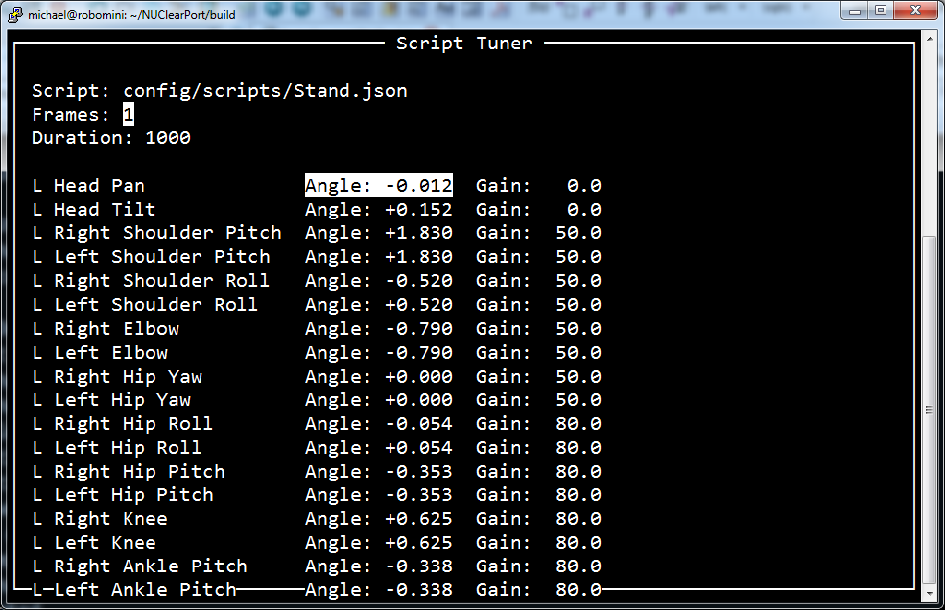
\includegraphics[width=1\textwidth]{./Images/tuner}

				Script Tuner is a module that provides an ncurses-based user interface for
				creating, editing and tweaking motion scripts. As it runs on the robot itself,
				it allows for movements to be previewed while they are being designed.
\end{document}
